\documentclass[25pt, landscape, paperwidth=48in, paperheight=36in, margin=0mm, innermargin=10mm, blockverticalspace=10mm, colspace=15mm, subcolspace=8mm]{tikzposter}
\usepackage[utf8]{inputenc}
\usepackage{graphicx}
\usepackage{amsmath}
\usepackage{booktabs}
\usepackage{xcolor}

% --- Custom Baylor University Colors ---
% Baylor Green: #154734, Baylor Gold: #FFB81C
\definecolor{BaylorGreen}{HTML}{154734}
\definecolor{BaylorGold}{HTML}{FFB81C}
\definecolor{White}{HTML}{FFFFFF}
\definecolor{Black}{HTML}{000000}

% --- Theme Definition ---
\definecolorstyle{BaylorStyle} {
    \colorlet{colorOne}{BaylorGreen}
    \colorlet{colorTwo}{BaylorGold}
    \colorlet{colorThree}{White}
}{
    % Background Colors
    \colorlet{backgroundcolor}{White}
    \colorlet{framecolor}{BaylorGold}
    % Title Colors
    \colorlet{titlebgcolor}{BaylorGreen}
    \colorlet{titlefgcolor}{BaylorGold}
    % Block Colors
    \colorlet{blocktitlebgcolor}{BaylorGreen}
    \colorlet{blocktitlefgcolor}{BaylorGold}
    \colorlet{blockbodybgcolor}{White}
    \colorlet{blockbodyfgcolor}{Black}
    % Innerblock Colors
    \colorlet{innerblocktitlebgcolor}{BaylorGold}
    \colorlet{innerblocktitlefgcolor}{Black}
    \colorlet{innerblockbodybgcolor}{White}
    \colorlet{innerblockbodyfgcolor}{Black}
}

\definetitlestyle{BaylorTitle}{
    width=\paperwidth, linewidth=0pt, innersep=30pt,
    titletotopverticalspace=0mm, titletoblockverticalspace=10mm
}{
    \begin{scope}[line width=\titlelinewidth]
        \draw[color=blocktitlebgcolor, fill=titlebgcolor]
        (\titleposleft,\titleposbottom) rectangle (\titleposright,\titlepostop);
    \end{scope}
}

\usetheme{Default}
\usecolorstyle{BaylorStyle}
\usetitlestyle{BaylorTitle}

% --- Title Information ---
\title{
    % The logo is placed in a zero-width box so it floats on the left without altering the center alignment of the text!
    \makebox[0pt][l]{\raisebox{-0.5\height}{\includegraphics[width=16cm]{figs/BU_BrandMark_Stacked_Gold.png}}}%
    % The text block uses the ENTIRE width of the poster to guarantee exact center alignment
    \begin{minipage}[c]{1.0\linewidth}
        \centering
        {\fontsize{110}{130}\selectfont \textbf{\textcolor{White}{AI-Enhanced Trace-Driven API Testing}}}\\[0cm]
        {\fontsize{110}{130}\selectfont \textbf{\textcolor{White}{with Comprehensive Microservice Validation}}}\\[0.6cm]
        {\fontsize{80}{100}\selectfont \textbf{Tingshuo Miao}}{\fontsize{55}{70}\selectfont \textbf{, PhD Candidate (Advisor: Dr. Eunjee Song)}}\\[-0.3cm]
        {\fontsize{60}{75}\selectfont \textbf{Department of Computer Science, Baylor University}}
    \end{minipage}
}
% Empty out standard metadata since we elegantly packed it all into the massive custom Title block above
\author{}
\institute{}
\titlegraphic{}

\begin{document}

\maketitle

% ----------------------------------------------------------------
% PURE 3-COLUMN LAYOUT
% ----------------------------------------------------------------
\begin{columns}

    % ==========================================
    % --- Column 1: Intro & Approach (Left) ---
    % ==========================================
    \column{0.25}
    
    \block{The Microservice Testing Challenge}{
        \Large
        Modern software relies heavily on \textbf{microservices}—a collection of small, specialized APIs that collaborate to fulfill complex user requests. While ensuring immense scalability, this architecture creates a massive testing blind spot:
        
        \vspace{0.8cm}
        % Stacked vertically for the narrow column
        \innerblock{The Integration Gap}{
            Testing individual services in isolation entirely misses catastrophic failures that only occur when passing complex data between multiple services during real user transactions.
        }
        
        \vspace{0.8cm}
        \innerblock{Workflow Fragility}{
            Trying to manually simulate end-to-end workflows is notoriously brittle. Invisible, temporary data dependencies consistently break traditional, rigid testing tools.
        }
    }

    \block{Our Novel Approach: Root API Mode}{
        \Large
        \innerblock{1. Extracting Entry Points}{
            Analyzes actual production traces to identify \textbf{Root APIs}---the public-facing "front doors" that trigger expansive internal service communications.
        }
        
        \vspace{0.7cm}
        \innerblock{2. AI-Driven Data Generation}{
            Uses Large Language Models (LLMs) and \textit{Smart Input Fetching} to synthesize highly realistic, semantically valid inputs targeting these Root APIs.
        }
        
        \vspace{0.7cm}
        \innerblock{3. The Sniper Strategy}{
            Introduces exactly one targeted error into a single root API while keeping surrounding data perfectly valid, isolating breaking points without noisy cascades.
        }
    }

    % ==========================================
    % --- Column 2: Architecture & Diagnosis (Center) ---
    % ==========================================
    \column{0.50}
    
    \block{System Architecture \& Pipeline}{
        \Large
        Our Trace-Driven pipeline follows an automated lifecycle. Tests are executed exclusively against the initial entry points, after which we capture the resulting backend traces.

        \vspace{0.8cm}
        \begin{tikzfigure}[Trace-driven testing pipeline]
            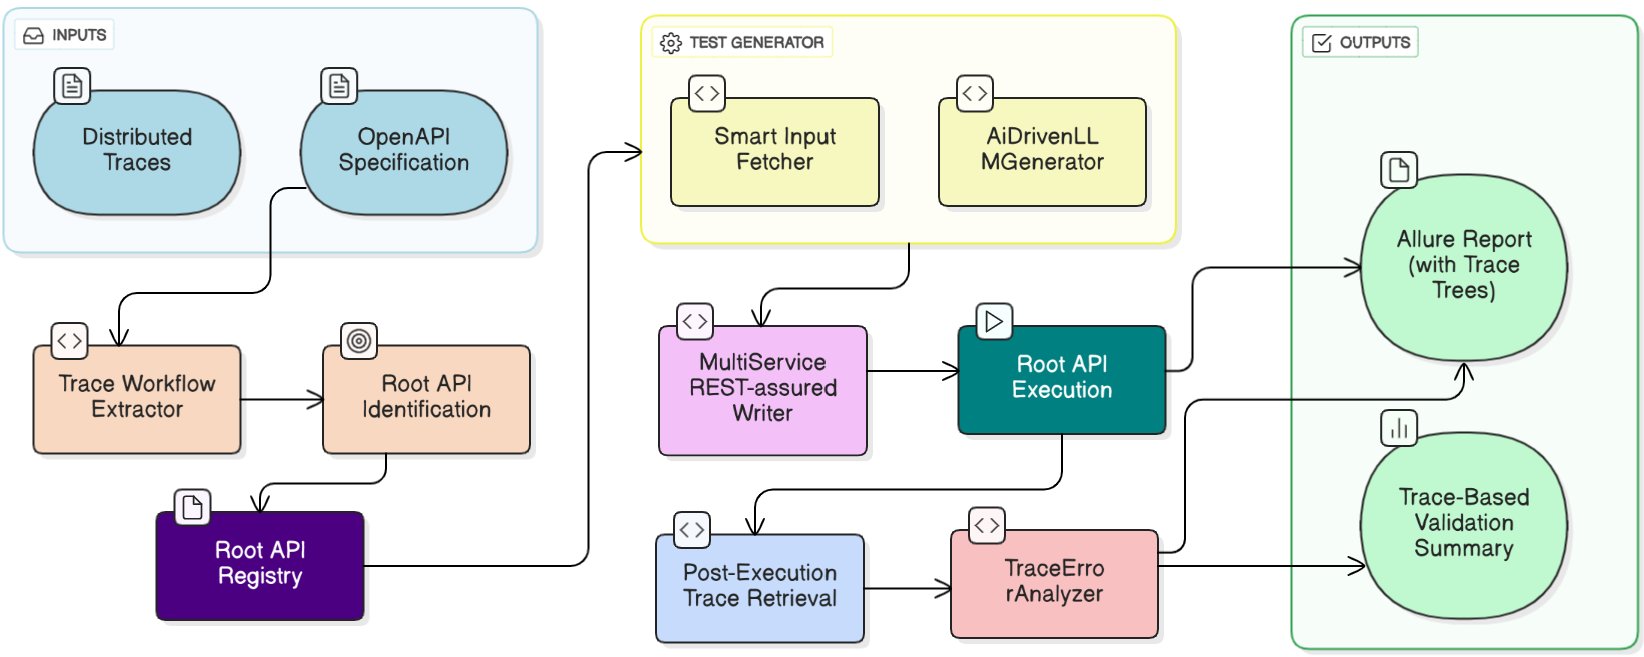
\includegraphics[width=0.85\linewidth]{figs/Res_flow.png}
        \end{tikzfigure}
        
        \vspace{0.8cm}
        By avoiding artificial simulation artifacts and monitoring real system behavior natively, our testing maintains perfect causal consistency.
    }

    \block{Trace-Driven Diagnosis \& Healing}{
        \Large
        \vspace{0.7cm}
        % In this wide 50% column, we place the two images perfectly side-by-side!
        \begin{minipage}[t]{0.48\linewidth}
            \vspace{0pt}
        By comparing intended inputs against post-execution distributed traces, our framework achieves a complete, hierarchical view of the system's true behavior.            \vspace{1cm}
            \begin{tikzfigure}[API call hierarchy visualization]
                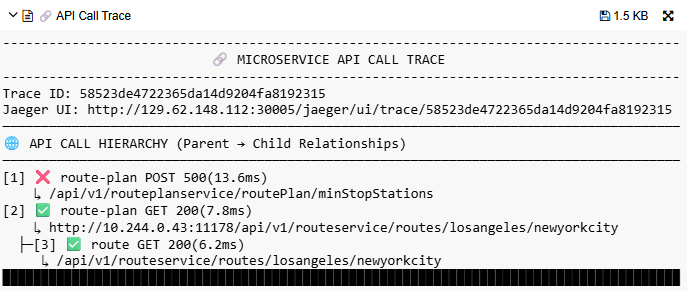
\includegraphics[width=0.95\linewidth]{figs/experiment/api_info.png}
            \end{tikzfigure}
            \vspace{1cm}
        \end{minipage}
        \hfill
        \begin{minipage}[t]{0.48\linewidth}
            \vspace{0pt}
                    When an error is detected deep within the microservice tree, our \textbf{AI Reasoning Engine} steps in. It correlates technical stack traces directly with trace telemetry to generate an \textit{Intelligent Analysis}.
            \vspace{1cm}
            \begin{tikzfigure}[AI-generated Root Cause Analysis]
                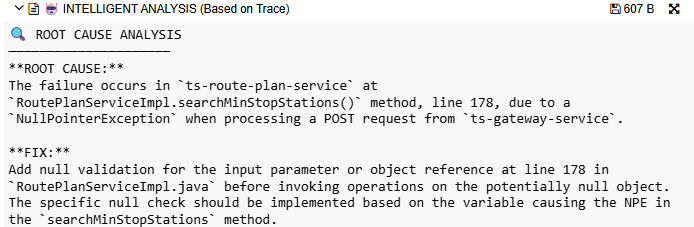
\includegraphics[width=0.95\linewidth]{figs/experiment/INTELLIGENT_ANALYSIS.png}
            \end{tikzfigure}
            \vspace{1cm}
        \end{minipage}
    }

    % ==========================================
    % --- Column 3: Results (Right) ---
    % ==========================================
    \column{0.25}
    
    \block{Key Results \& Conclusion}{
        \Large
        \textbf{Evaluation:} We evaluated our framework against industry-standard tools (\textsc{RESTest} and EvoMaster) by injecting 10 complex faults into the TrainTicket microservice system.
        
        \vspace{1.0cm}
        \begin{center}
            \renewcommand{\arraystretch}{1.8}
            \resizebox{1.0\linewidth}{!}{
            \begin{tabular}{l l c}
            \toprule
            \textbf{Testing Tool} & \textbf{Strategy} & \textbf{Faults Detected} \\
            \midrule
            \textsc{RESTest} & Static Specification Analysis & 3 / 10 \\
            \textsc{EvoMaster} & Search-Based S/W Testing (SBST) & 6 / 10 \\
            \textbf{Our Approach} & \textbf{Trace-Driven AI Synthesis} & \textbf{10 / 10} \\
            \bottomrule
            \end{tabular}
            }
        \end{center}

        \vspace{1.5cm}
        \innerblock{Conclusion}{
            By anchoring executions at authentic entry points and utilizing powerful post-execution trace analysis, our system provides \textbf{superior 100\% fault detection}, translating opaque failures directly into actionable, code-level fixes.
        }
    }

    \block{Future Work}{
        \Large
        \textbf{Step API Test Generation:} Extend test synthesis to target internal step APIs (single inter-service operations/spans) to directly validate internal microservice boundaries.\\[0.3cm]
        \textbf{Optimize AI Efficiency:} Reduce the 25-hour execution overhead via model fine-tuning and semantic caching.\\[0.3cm]
        \textbf{CI/CD Integration:} Enable dynamic test suite adaptation based on live production telemetry.\\[0.3cm]
        \textbf{Stateful Concurrency:} Extend orchestrator to validate distributed race conditions across multi-root sequences.
    }

\end{columns}

% --- Sleek Edge-to-Edge Footer Bar ---
\node[
    anchor=south,
    minimum width=\paperwidth,
    minimum height=4cm,
    fill=titlebgcolor,
    text=titlefgcolor,
] at (0, -0.5\paperheight) {
    \makebox[0.96\paperwidth][c]{
        {\fontsize{35}{45}\selectfont \textbf{BaylorECS Summit 2026}}
        \hfill 
        {\fontsize{35}{45}\selectfont \textbf{Contact: Tingshuo\_Mia2@baylor.edu}}
    }
};

\end{document}
